\documentclass[12 pt]{exam}
\usepackage{graphicx, enumitem, amsmath, amssymb}
\graphicspath{ {./images/} }
\usepackage{tikz, pgfplots}
\pgfplotsset{compat=1.16}
\usetikzlibrary{shapes,arrows}
%\usepackage{Minion Pro}
\printanswers

\title{2.3 Cost Minimization - Practice Problems (Answers)}
\author{Ryan Safner}
\date{ECON 306 - Fall 2019}

\begin{document}

\maketitle

Your firm can use labor $l$ and capital $k$ to produce output according to the production function:
$$q=4lk$$


The marginal products are:

$$\begin{aligned}
MP_l &=4k \\
MP_k &=4l \\ \end{aligned}$$

Suppose you  need to produce 144 units, the price of labor is \$10, and the price of capital is \$40. 

\begin{questions}

\question What is the least-cost combination of labor and capital that produces 144 units of output?

  \begin{solution}
  	Use the definition of the optimum: 
\begin{align*}
MRTS_{l,k}&=\frac{w}{r} & & \text{Definition of the optimum}\\
\frac{MP_l}{MP_k}&=\frac{w}{r} && \text{Definition of MRTS on left}\\
\frac{4k}{4l} &=\frac{(10)}{(40)} & & \text{Plugging in what we know}\\
		\frac{k}{l}&=\frac{1}{4} && \text{Simplifying}\\
	k&=\frac{1}{4}l && \text{Multiplying both sides by} l\\	
\end{align*}

So we know that we will be using 1 unit of capital for every 4 workers (this should make sense, as capital is 4 times as expensive as labor). This is the optimal ratio of inputs. 

To find the exact quantities of $l$ and $k$, use the production function:

\begin{align*}
q&=4lk & & \text{The production function}\\
144&4l(\frac{1}{4}l) & & \text{Plugging in what we are given and what we found}\\
144&=l^2 & & \text{Multiplying}\\
12&=l & & \text{Square rooting both sides}\\
\end{align*}

Now that we know the quantity of labor, we can use our knowledge of the ratio of labor to capital to find the optimal quantity of capital. 
\begin{align*}
k&=\frac{1}{4}l\\
k&=\frac{1}{4}(12)\\
k&=3\\ 	
\end{align*}

So using 12 workers and 3 units of capital produces 144 units of output at the lowest total cost.
\end{solution}

\question How much does this combination cost?

\begin{solution}

\begin{align*}
wl+rk&=C && \text{The isocost line equation}\\
10(12)+40(3)&=C && \text{Plugging in what we know (prices) and what we found}\\
120+120&=C && \text{Multiplying}\\
240&=C && \text{Adding}\\
\end{align*}

The total cost of using 12 workers and 3 units of capital at current prices is \$240.

\end{solution}

\question Does this technology experience constant returns, increasing returns, or decreasing returns to scale?

\begin{solution}

Simply plug in combinations of labor and capital that change at the same rate, and see at what rate output changes. For example, with 1 worker, 1 unit of capital, output is:

\begin{align*}
q&=4lk\\
q&=4(1)(1)\\
q&=4
\end{align*}

If we now *double* all inputs, so that we use 2 workers and 2 units of capital, output is

\begin{align*}
q&=4lk\\
q&=4(2)(2)\\
q&=16
\end{align*}

Output has quadrupled from 4 to 16, from a doubling of all inputs. Therefore, this technology exhibits increasing returns to scale.

There is a shortcut that we could use, because this function is in Cobb-Douglas format (inputs and \emph{multiplied} by each other, and each raised to an exponent), we can simply sum the exponents:

$$q=4l^{1}k^{1}$$
$$1+1=2$$

Because the exponents sum to a number greater than one, this technology is increasing returns. Be careful, this shortcut method \emph{only} works for Cobb-Douglas functions!

\end{solution}

\begin{center}
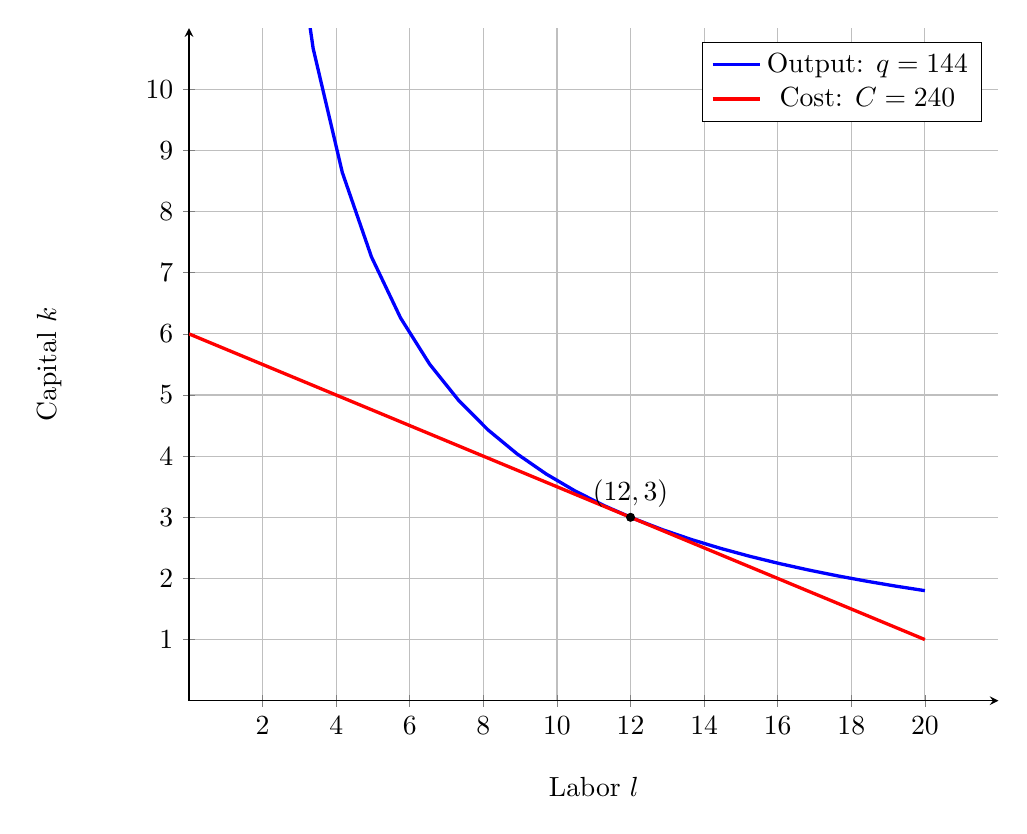
\begin{tikzpicture}
\begin{axis}[clip=true,
 			scale=1.5,
		axis lines=middle, 
		enlarge x limits={rel=0.1, upper},
		enlarge y limits={rel=0.1, upper},
		every axis y label/.style={at={(axis description cs:-0.2,0.5)},rotate=90,anchor=north},
		every axis x label/.style={at={(axis description cs:0.5,-0.1)},anchor=north},
	%legend pos=outer north east,
	xlabel=Labor $l$,
	ylabel=Capital $k$,
	shader=flat,
	xtick={0,2,4,...,20},
	ytick={0,1,2,...,10},
	grid=major,
	ymin=0,
	xmin=0,
	ymax=10,
	xmax=20,
]
	\addplot[domain=1:20, samples=25, very thick, color=blue]{36/x};
	\addlegendentry{Output: $q=144$};
	\addplot[domain=0:20, samples=25, very thick, color=red]{6-0.25*x};
	\addlegendentry{Cost: $C=240$};
	\draw[fill=black] (axis cs:12,3)circle(0.05cm)node[above]{$(12,3)$};
\end{axis}
\end{tikzpicture}
\end{center}

\end{questions}

\end{document}